% ---------------------------------------------------------------------------
% Where electromagnetically induced transparency lives, and where it inverts,
% for the NV(-) spin-Lambda channel in diamond.
%
% Physical Review A manuscript.  Build:
%   pdflatex nv_eit_pra && bibtex nv_eit_pra && pdflatex nv_eit_pra x2
% Figures: ../results/figures/*.pdf, produced by ../src/make_figures.py
% ---------------------------------------------------------------------------
\documentclass[
  reprint,
  amsmath,amssymb,
  aps,pra,
  superscriptaddress,
  floatfix,
]{revtex4-2}

\usepackage{graphicx}
\usepackage{bm}
\usepackage{siunitx}
\usepackage{xcolor}
\definecolor{linknavy}{rgb}{0.10,0.22,0.45}
\usepackage[colorlinks=true,linkcolor=linknavy,citecolor=linknavy,
            urlcolor=linknavy]{hyperref}

\graphicspath{{../results/figures/}}

\newcommand{\Bperp}{B_{\perp}}
\newcommand{\dchi}{\delta\chi_{S}}
\newcommand{\Acut}{A_{\mathrm{cut}}}
\newcommand{\Afull}{A_{\mathrm{full}}}
\newcommand{\Gxy}{\Gamma_{XY}}
\newcommand{\ms}{m_{s}}

\begin{document}

\title{Where electromagnetically induced transparency lives, and where it
inverts, in the nitrogen--vacancy spin-$\Lambda$ channel}

\author{Risei Abe}
\affiliation{Department of Electrical and Electronic Engineering,
Institute of Science Tokyo, Tokyo, Japan}

\date{\today}

\begin{abstract}
Electromagnetically induced transparency (EIT) has been observed in
nitrogen--vacancy (NV$^{-}$) ensembles at low temperature, but no microscopic
account exists of why it disappears on warming, how far external control can
recover it, or what remains at room temperature. We resolve the weak-probe
response of the NV$^{-}$ zero-phonon-line spin-$\Lambda$ channel with the full
nine-level Lindblad generator and classify every point of the
temperature--transverse-field plane by three criteria applied together: the
sign of the coherence-mediated contrast, the lineshape of the control-on
absorption, and an Akaike model comparison against Autler--Townes splitting.
The region supporting genuine transparency is a closed island. It requires a
transverse field $\Bperp \gtrsim \SI{0.15}{\tesla}$ to open the Raman pathway
at all; it is bounded below near \SI{22}{\kelvin} by an Autler--Townes
crossover, and above near \SI{90}{\kelvin}--\SI{95}{\kelvin} by phonon-driven
collapse of the leading Raman path, which costs four and a half orders of
magnitude of contrast between \SI{30}{\kelvin} and \SI{100}{\kelvin}. Above
$103\,[97,\,108]~\si{\kelvin}$ the response changes sign: the control field no
longer induces transparency but induces absorption. Raising $\Bperp$ from
\SI{0.15}{\tesla} to \SI{0.5}{\tesla} moves the boundary by less than
\SI{2}{\kelvin}, so the transverse field opens the channel without buying
temperature. Converting to laboratory observables on a single detection chain,
the sign reversal itself lies inside the detectable region --- reachable in
seconds of integration --- whereas at room temperature the residual contrast
of $\sim\!10^{-9}$ is unreachable at any integration time once a realistic
technical-noise floor is imposed. We also delimit where the reduced
kernel widely used for such estimates may be trusted: it reproduces the
boundary temperatures but not the contrast magnitudes, and it fails
qualitatively, including in sign, below \SI{40}{\kelvin} and above
\SI{90}{\kelvin}.
\end{abstract}

\maketitle

% ===========================================================================
\section{Introduction}
% ===========================================================================

Electromagnetically induced transparency renders an absorbing medium
transparent to a weak probe by destructive interference of excitation
pathways opened by a strong control field~\cite{M2005C01}. In atomic vapours
the mechanism is textbook. In solids it is not: the same $\Lambda$-shaped
level diagram can yield a deep transparency window in one material and
nothing at all in another, because real emitters carry many excited branches,
several dissipative channels, and material-specific selection rules that the
three-level picture does not contain.

The negatively charged nitrogen--vacancy centre in diamond is the most
thoroughly characterised of these systems~\cite{M2013S07}. Coherent population
trapping of single NV spins~\cite{C2006S02} and EIT in NV
ensembles~\cite{V2013S01} have both been demonstrated at cryogenic
temperature, and the appeal of extending them upward is obvious: an
all-optical, room-temperature coherent interface in a material that already
supports room-temperature spin readout. What has been missing is an account
of \emph{why} the low-temperature effect does not survive warming. The usual
explanation --- that dephasing grows and washes the feature out --- is
incomplete, because it predicts only a monotonic fading. It does not predict
a lower temperature bound, it does not predict a threshold in transverse
field, and it does not predict a change of sign. All three occur.

We compute the weak-probe response of the NV$^{-}$ zero-phonon-line
spin-$\Lambda$ channel without adiabatic elimination, using the full
nine-level Lindblad generator, over the temperature--transverse-field plane.
The organising quantity is not the total susceptibility but the part of it
carried by the targeted ground-state coherence, isolated by an algebraic
counterfactual: the sector-resolved correction $\dchi$. This distinction is
not cosmetic. A vanishing \emph{total} susceptibility is the signature of
ideal EIT, not of its absence, so a criterion built on the total response has
the sign of the conclusion backwards. Section~\ref{sec:theory} makes the
construction precise.

Three results follow. First, the transparency region is a closed island in
the $(T,\Bperp)$ plane rather than a half-space below some temperature
(Sec.~\ref{sec:phase}). Second, the transverse field is a switch and not a
dial: it must exceed a threshold before there is any channel, and once open,
further field buys essentially no temperature headroom
(Sec.~\ref{sec:bperp}). Third, above $\sim\!\SI{103}{\kelvin}$ the
coherence-mediated response inverts, so that the control field increases the
probe absorption; this inversion is not a vanishing remnant but a signal that
a realistic experiment can resolve in seconds, whereas the room-temperature
residual cannot be resolved at all (Sec.~\ref{sec:observables}).

Because a claim of this kind stands or falls on the validity of the model that
produced it, Sec.~\ref{sec:audit} reports the audit in full, including where
the reduced description that is commonly used for such estimates --- and that
we ourselves use for the uncertainty propagation --- may and may not be
trusted. The general classification of dissipative response orders that the
present analysis instantiates is developed separately and is not assumed here.

% ===========================================================================
\section{Response theory and the object that is classified}
\label{sec:theory}
% ===========================================================================

\subsection{Model}

The NV$^{-}$ ground manifold is the $^{3}A_{2}$ spin triplet with
zero-field splitting $D_{gs}=\SI{2.877}{\giga\hertz}$; the optically
connected excited manifold is the six-dimensional $^{3}E$ orbital doublet,
carrying spin--orbit, spin--spin, transverse strain and Zeeman
terms~\cite{A2009S03,G2017S08}. We retain both manifolds in full, giving nine
levels once the spectator ground sublevel is included, and evolve them with a
time-independent Lindblad generator in the rotating frame,
%
\begin{equation}
\dot\rho=\mathcal{L}(\rho)
=-i[H,\rho]+\sum_{\mu}\Big(L_{\mu}\rho L_{\mu}^{\dagger}
-\tfrac12\{L_{\mu}^{\dagger}L_{\mu},\rho\}\Big).
\label{eq:gksl}
\end{equation}
%
The jump operators are spin-conserving radiative decay from each excited
branch, phonon-induced orbital hopping $E_{x}\!\leftrightarrow\!E_{y}$ at rate
$k_{\mathrm{orb}}(T)$, ground-state relaxation, and ground-state dephasing.
Intersystem crossing to the singlet and $^{14}$N hyperfine structure are
available as structural toggles and are used in the audit of
Sec.~\ref{sec:audit}.

The temperature enters through $k_{\mathrm{orb}}(T)$, taken from the
measured photophysics of single NV centres~\cite{J2023S06} and cross-checked
against three alternative rate models as a systematic
(Sec.~\ref{sec:boundary}). The essential point for what follows is a property
of the \emph{coherence} block rather than of populations: a jump confined to
the excited manifold, which merely shuffles population between $E_{x}$ and
$E_{y}$ and removes none, nevertheless acts on every optical coherence as
pure loss. Writing $\sigma=P_{e}\rho P_{g}$ for the optical-coherence block,
%
\begin{equation}
P_{e}\,\mathcal{D}[L_{\mu}](\rho)\,P_{g}
=-\tfrac12 L_{\mu}^{\dagger}L_{\mu}\,\sigma ,
\qquad L_{\mu}=P_{e}L_{\mu}P_{e},
\label{eq:pureloss}
\end{equation}
%
because the recycling term cannot connect the rectangular block to itself.
Orbital hopping is therefore a decoherence channel for the Raman pathway even
though it conserves excited-state population, and this is the microscopic
origin of the collapse reported below. One consequence deserves emphasis
because it is a recurring source of factor errors: for symmetric two-way
hopping at rate $k$ the population imbalance relaxes at
$\Gxy=2k$, while each optical coherence is damped at $k/2=\Gxy/4$. The rate
that enters Eq.~\eqref{eq:pureloss} is a quarter of the orbital relaxation
rate usually quoted.

\subsection{The sector-resolved correction}

Let the first-order response be organised into the optical-coherence vector
$x$ and the targeted ground coherence $s=\rho^{(1)}_{g_{2}g_{1}}$,
%
\begin{equation}
\begin{pmatrix} A & B\\ C & G_{g}\end{pmatrix}
\begin{pmatrix} x\\ s\end{pmatrix}
=\begin{pmatrix} b_{p}\\ 0\end{pmatrix}.
\label{eq:block}
\end{equation}
%
Eliminating $x$ --- so that $G_{g}$ is never inverted and the ideal
ground-coherence limit is retained --- gives the probe response as a Schur
complement. We define the \emph{pathway-cut} counterfactual
$\chi^{(S)}_{\mathrm{cut}}$ by setting $B=C=0$ while holding $A$, $G_{g}$, the
source, the detector and the zeroth-order state fixed, and the
sector-resolved correction
%
\begin{equation}
\dchi \equiv \chi_{\mathrm{full}}-\chi^{(S)}_{\mathrm{cut}}
= \chi_{0}\, d^{\dagger}A^{-1}B\,S_{g}^{-1}\,CA^{-1}b_{p},
\label{eq:dchi}
\end{equation}
%
with $S_{g}=G_{g}-CA^{-1}B$. Throughout we report the dimensionless contrast
%
\begin{equation}
C \;=\; \frac{\Acut-\Afull}{\Acut},
\label{eq:contrast}
\end{equation}
%
where $\Afull$ and $\Acut$ are the control-on absorptions with and without the
ground-coherence pathway. With this convention $C>0$ means the pathway
\emph{reduces} absorption --- transparency --- and $C<0$ means it increases
it.

Two properties of Eq.~\eqref{eq:dchi} matter for the interpretation of every
figure below. It is an algebraic counterfactual, not a control-off
measurement: switching the control off would also change optical pumping,
light shifts and the steady state, and would therefore not isolate the
coherence pathway. And it is the correct object to test, because
$\chi_{\mathrm{full}}=0$ is what \emph{perfect} EIT looks like. In the ideal
three-level limit the total response vanishes while $\dchi$ is maximal; a
criterion phrased on the total susceptibility would report that case as an
absence of EIT.

Both statements are exact in the case where the answer is already known. For
one excited state and scalar dipoles the blocks are scalars: $A=\gamma_{31}+i
\delta_{p}$, $G_{g}=\gamma_{21}+i(\delta_{p}-\delta_{c})$,
$BC=-|\Omega_{c}|^{2}/4\equiv-\beta$ and $b_{p}=i\Omega_{p}/2$, and
Eq.~\eqref{eq:block} collapses to
%
\begin{equation}
\rho_{e1}=\frac{b_{p}}{A+\beta/G_{g}}
=\frac{i\Omega_{p}/2}
{\gamma_{31}+i\delta_{p}
+\dfrac{|\Omega_{c}|^{2}/4}{\gamma_{21}+i(\delta_{p}-\delta_{c})}},
\label{eq:textbook}
\end{equation}
%
which is the standard weak-probe EIT coherence~\cite{M2005C01} term by term.
No adiabatic elimination is used in obtaining it. Setting
$\delta_{p}=\delta_{c}=0$ and $\gamma_{21}\to0$ then gives
$\chi_{\mathrm{full}}=0$ and $\dchi/\chi^{(S)}_{\mathrm{cut}}=-1$: the total
response vanishes while the sector-resolved correction is maximal, which is
the preceding paragraph's claim as an identity rather than an assertion. The
three reductions are verified symbolically in
\texttt{calculations/symbolic/verify\_lambda\_reduction.py}.

\subsection{Classification}

At each point of the $(T,\Bperp)$ plane we scan the two-photon detuning with
an adaptive window --- the feature width varies over three orders of
magnitude across the plane --- and assign one of four labels using the sign of
the peak contrast, the containment of the feature, and a model comparison of
the control-on lineshape. The lineshape test follows Anisimov, Dowling and
Sanders~\cite{P2011C10}: the absorption profile is fitted with an EIT
(interference) model and an Autler--Townes (doublet) model, together with
Lorentzian and Fano alternatives, and the verdict is fixed by
$\Delta\mathrm{AIC}=\mathrm{IC}_{\mathrm{ATS}}-\mathrm{IC}_{\mathrm{EIT}}$
with a robust gate at $|\Delta\mathrm{AIC}|\ge 6$. A point is labelled
\emph{genuine transparency} only if $C>0$, the feature is contained in its
window, $|C|$ exceeds the detection floor, and the lineshape is robustly EIT.
A negative $C$ is labelled \emph{control-induced absorption}; a robustly ATS
lineshape is labelled Autler--Townes; everything else is \emph{unresolved},
which includes both sub-threshold features and genuinely inconclusive
lineshapes.

Requiring all three criteria jointly is what separates this classification
from a contrast map. A large $|C|$ alone is not evidence of transparency: $C$
is a ratio, and where the probe leg is nearly closed the denominator is small,
so $|C|$ can be large while the absolute absorption change is negligible ---
or, as we find at low field, while the control is in fact turning absorption
\emph{on}. We therefore record the absolute absorptions alongside $C$
everywhere.

% ===========================================================================
\section{The transparency island}
\label{sec:phase}
% ===========================================================================

\begin{figure}[t]

\includegraphics[width=\columnwidth]{fig1_level_scheme.pdf}
\caption{(a) The NV$^{-}$ spin-$\Lambda$ channel. Probe and control address
two ground spin sublevels through the $^{3}E$ orbital doublet. Because the
optical dipole is orbital, the two legs reach orthogonal spin states and the
leading Raman vertex is closed at $\Bperp=0$; a transverse field mixes the
ground sublevels and opens it. Phonon-induced hopping $\Gxy(T)$ between the
excited branches damps the pathway.
(b) Optical-coherence damping $\gamma_{\mathrm{oc}}(T)$ over the range studied,
with the transverse strain splitting marked for scale. The island boundaries
found in Sec.~\ref{sec:phase} are indicated.}
\label{fig:levels}
\end{figure}

\begin{figure*}[t]
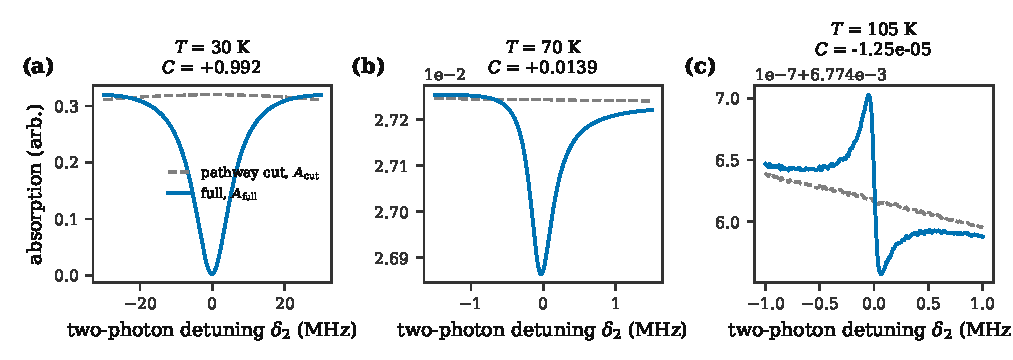
\includegraphics[width=\textwidth]{fig2_spectra.pdf}
\caption{Full-Liouvillian absorption spectra at the candidate field
$\Bperp=\SI{0.232}{\tesla}$, with the ground-coherence pathway intact
($\Afull$, solid) and cut ($\Acut$, dashed). (a) At \SI{30}{\kelvin} the
pathway removes essentially all of the sector absorption. (b) At
\SI{70}{\kelvin} a per-cent-level transparency survives. (c) At
\SI{105}{\kelvin} the two curves have crossed: the pathway now \emph{adds}
absorption, and the contrast has changed sign.}
\label{fig:spectra}
\end{figure*}

Figure~\ref{fig:phase} is the central result. Two features of it are not
anticipated by a dephasing-washout picture.

\emph{A threshold in transverse field.} At $\Bperp=0$ there is no usable
transparency at any temperature. This is not an artefact of small numbers: the
optical dipole is orbital, so with unmixed ground sublevels the two legs of
the $\Lambda$ terminate on orthogonal spin states and the leading Raman
vertex vanishes identically. What survives at zero field is a small residual
pathway through spin mixing inside $^{3}E$, of order $10^{-5}$ in contrast at
\SI{70}{\kelvin}, which is a different pathway and which we separate
explicitly in Sec.~\ref{sec:bperp}. Genuine transparency appears only for
$\Bperp\gtrsim\SI{0.15}{\tesla}$.

\emph{A lower temperature bound.} Below about \SI{22}{\kelvin} the region
closes again. As the optical line narrows on cooling, the fixed control Rabi
frequency $\Omega_{c}=\SI{0.1}{\giga\hertz}$ becomes large compared with the
optical-coherence damping, and the response crosses into the Autler--Townes
regime: at \SI{20}{\kelvin} the lineshape test returns robust ATS at the
larger fields and the contrast is negative at the smaller ones, with a wide
feature (FWHM $\sim\SI{70}{\mega\hertz}$ at \SI{10}{\kelvin}) that is a
dressed-state doublet rather than an interference window. The transparency
region is therefore an island, bounded below by a control-power crossover and
above by dissipation.

Between those bounds the collapse with temperature is steep. At
$\Bperp=\SI{0.232}{\tesla}$ the contrast falls from $0.99$ at
\SI{30}{\kelvin} through $0.58$ at \SI{50}{\kelvin}, $1.4\times10^{-2}$ at
\SI{70}{\kelvin} and $1.5\times10^{-4}$ at \SI{90}{\kelvin} to
$2.1\times10^{-5}$ at \SI{100}{\kelvin} --- four and a half orders of
magnitude over \SI{70}{\kelvin} --- and then changes sign. The upper edge of
the transparency label sits at \SI{90}{\kelvin} for
$\Bperp\le\SI{0.25}{\tesla}$ and \SI{95}{\kelvin} above it, with a band of
lineshape-inconclusive points immediately beyond, so the boundary is not
sharp; the sign reversal that follows is.

\subsection{Why the sign reverses: a damping-induced phase slip}
\label{sec:phaseslip}

The sign of $\dchi$ is set by the phase of the Raman vertex product
$K_{12}K_{21}$ relative to the ground-coherence denominator
$\gamma_g+\beta S_2$ in Eq.~\eqref{eq:dchi}: writing
$K_{12}K_{21}/(\gamma_g+\beta S_2)=r\,e^{i\phi}$ with $r>0$, the correction is
$\dchi\propto-r\cos\phi$, so the pathway is transparency-producing while
$|\phi|<90^\circ$ and absorption-producing once $|\phi|$ exceeds it. At the
candidate field, $\arg(K_{12}K_{21})$ runs from $-0.1^\circ$ at
\SI{30}{\kelvin} through $-17.0^\circ$ at \SI{70}{\kelvin} and $-62.7^\circ$
at \SI{90}{\kelvin} to $-89.3^\circ$ at \SI{100}{\kelvin}, while the
denominator's phase stays small ($\lesssim15^\circ$ throughout); the combined
phase $\phi$ crosses $-90^\circ$ between \SI{100}{\kelvin} and
\SI{103}{\kelvin}, exactly where the numerically observed sign reversal sits.

The mechanism is the phase lag of a damped driven resonance. $K_{12}$ and
$K_{21}$ are matrix elements of the resolvent
$G=[\gamma_{\mathrm{oc}}(T)\,I+i2\pi(H-zI)]^{-1}$: while the
optical-coherence damping $\gamma_{\mathrm{oc}}(T)$ is small compared with the
excited-state splittings, $G$ responds essentially in phase with the drive and
the Raman pathway interferes \emph{destructively} with the direct absorption
path, which is transparency. As $\gamma_{\mathrm{oc}}(T)$ grows past that
internal scale --- here the transverse-strain splitting
$\delta\sim\SI{1.7}{\giga\hertz}$, reached once phonon-induced orbital hopping
brings $\gamma_{\mathrm{oc}}(T)\gtrsim\delta$ near \SI{100}{\kelvin} --- the
resolvent lags the drive by more than a quarter cycle, and the same
interference term that used to cancel absorption now reinforces it:
destructive interference has become constructive, i.e.\ the coherent pathway
behaves as electromagnetically induced absorption rather than transparency. No
new parameter or mechanism is introduced; the reversal is the phase response
of a resonance being pushed through overdamping by the same
temperature-dependent rate that drives the amplitude collapse of
Sec.~\ref{sec:phase}, which is why the two occur within one narrow temperature
interval rather than as independent features.

\begin{figure*}[t]

\includegraphics[width=\textwidth]{fig3_phase_diagram.pdf}
\caption{(a) Classification of the $(T,\Bperp)$ plane from the full nine-level
Liouvillian, using sign, lineshape containment and the EIT/ATS model
comparison jointly. Genuine transparency occupies a closed island: it requires
$\Bperp\gtrsim\SI{0.15}{\tesla}$, closes below $\sim\SI{22}{\kelvin}$ through
an Autler--Townes crossover, and closes above
$\SI{90}{\kelvin}$--$\SI{95}{\kelvin}$ through phonon-driven collapse.
(b) The same plane on a single signed scale: blue is $C>0$ (transparency),
red is $C<0$ (control-induced absorption), and colour depth is $|C|$ on a
symmetric-log axis. Fixed parameters: $B_{z}=\SI{5}{\milli\tesla}$,
$\Omega_{c}=\SI{0.1}{\giga\hertz}$, transverse strain
$\delta=\SI{1.683}{\giga\hertz}$.}
\label{fig:phase}
\end{figure*}

% ===========================================================================
\section{How the transverse field opens the pathway}
\label{sec:bperp}
% ===========================================================================

That a transverse field opens the channel is expected on symmetry grounds:
$\Bperp$ mixes the ground spin sublevels and thereby supplies the spin overlap
that the orbital dipole cannot. Because the mixing enters once in each leg of
the $\Lambda$, and the sector-mediated response is bilinear in the two Raman
vertices, the leading behaviour should be $C \simeq C_{\mathrm{res}} +
a\Bperp^{2}$, with $C_{\mathrm{res}}$ the field-independent residual pathway
through $^{3}E$ spin mixing.

The field range over which that law can be tested is bounded from both sides,
and narrowly. From above, the mixing ceases to be perturbative once the ground
Zeeman energy reaches the zero-field splitting, $\gamma_{e}\Bperp = D_{gs}$ at
$\Bperp=\SI{0.103}{\tesla}$; we take $\SI{0.031}{\tesla}$, three tenths of
that, as the ceiling of the perturbative window. From below, the fit needs the
opened part to stand clear of $C_{\mathrm{res}}$, which happens near
$\SI{0.008}{\tesla}$ at these temperatures. Less than a decade of field
separates the two. Note also that $C_{\mathrm{res}}$ cannot be read off at
$\Bperp=0$: that point is structurally degenerate and does not join smoothly
onto the small-field plateau, so the residual has to be a fitted parameter,
which is what including the plateau points in the fit constrains.

Fitting $C=C_{\mathrm{res}}+a\Bperp^{n}$ on a dense grid inside that window
separates the temperatures cleanly, and we report the separation rather than
an average over it. At \SI{85}{\kelvin} the exponent is stable against the
choice of upper cutoff --- it varies by $0.25$ over cutoffs from
\SI{0.022}{\tesla} to \SI{0.046}{\tesla}, with no monotone trend (Spearman
$\rho=-0.05$) --- and equals
%
\begin{equation}
n(\SI{85}{\kelvin}) = 2.11 \pm 0.08 ,
\end{equation}
%
which is the expected quadratic opening. At \SI{70}{\kelvin} and
\SI{55}{\kelvin} it is not stable: the fitted exponent drifts monotonically
downward with the cutoff ($\rho=-0.97$ at both, spanning $0.65$ and $0.86$
respectively), running from $2.7$--$3.0$ at the smallest usable cutoff through
$2$ near $\Bperp\approx\SI{0.04}{\tesla}$. A genuine power law shows a plateau
against the fitting window; a crossover shows exactly this drift.
Figure~\ref{fig:bperp}(b) displays the distinction directly. We therefore
claim the quadratic law at \SI{85}{\kelvin} and above, and state that it is
not resolvable at the cold end of the island.

Two controls establish that the drift belongs to the physics of the pathway
and not to the way it is interrogated. Varying the control Rabi frequency over
a factor of ten, $\Omega_{c}=0.03$ to \SI{0.3}{\giga\hertz}, moves the
\SI{70}{\kelvin} exponent from $2.664$ to $2.628$ --- that is, not at all
beyond the fit error. And fitting the absolute signal
$\Delta A=\Acut-\Afull$, which carries no field-dependent denominator, instead
of the ratio $C$ returns the same exponent ($2.70$ against $2.63$ at
\SI{70}{\kelvin}), so the excess above $2$ is not an artefact of normalising
by a quantity that itself varies with field. Together with the archived
room-temperature campaign, which returns $n=2.03$--$2.18$ where the dynamic
range is largest, the picture is that the opening is quadratic in its
asymptotic regime and that the cold end of the island simply does not reach
that regime before the mixing saturates.

The practical consequence does not depend on the exponent. $\Bperp$ behaves as
a switch rather than a dial: Sec.~\ref{sec:boundary} shows that raising it
from \SI{0.15}{\tesla} to \SI{0.5}{\tesla} moves the temperature boundary by
under \SI{2}{\kelvin}. The field is necessary to have a channel at all, and
once the channel is open the boundary is set by dissipation. This is the sense
in which the transverse-field route is not a recovery mechanism for
high-temperature EIT: it changes the prefactor of a suppressed response, not
the temperature at which the suppression sets in.

\begin{figure*}[t]

\includegraphics[width=\textwidth]{fig5_bperp_scaling.pdf}
\caption{Opening of the Raman pathway with transverse field, full
Liouvillian. (a) Sector contrast against $\Bperp$; solid curves are fits of
$C=C_{\mathrm{res}}+a\Bperp^{n}$ inside the perturbative window, whose ceiling
$B_{\mathrm{pert}}$ and the full-mixing field $\gamma_{e}\Bperp=D_{gs}$ are
marked. (b) The fitted exponent against the upper fitting cutoff. A power law
appears as a plateau and a crossover as a drift: \SI{85}{\kelvin} plateaus at
the expected $n=2$, while \SI{70}{\kelvin} and \SI{55}{\kelvin} drift
monotonically and do not determine an exponent.}
\label{fig:bperp}
\end{figure*}

% ===========================================================================
\section{Where the boundary lies, and how well it is known}
\label{sec:boundary}
% ===========================================================================

A boundary temperature quoted as a single number would misrepresent what is
known. We propagate the experimental and model uncertainty by Monte Carlo:
log-normal priors on the orbital-hopping and radiative rate scales, a normal
prior on the transverse strain, priors on both field components, a
log-uniform prior on the ground decoherence, a prior on the control Rabi
frequency, polarization-angle errors, and --- separately from the rate scales,
which is where earlier treatments folded it --- a log-uniform prior on an
additional optical linewidth representing spectral diffusion. The four
phonon-rate models enter as a discrete systematic rather than a single
extrapolation.

Two thresholds are reported: $T_{1\%}$, where the contrast falls through
$10^{-2}$, and $T_{\mathrm{sign}}$, where it changes sign. At the candidate
field, from the full Liouvillian,
%
\begin{align}
T_{1\%} &= 74\,[70,\,78]~\si{\kelvin},\\
T_{\mathrm{sign}} &= 103\,[97,\,108]~\si{\kelvin},
\end{align}
%
as 68\% intervals. The field dependence separates sharply into two regimes.
For $\Bperp\le\SI{0.10}{\tesla}$ both thresholds collapse to
\SI{27}{\kelvin}--\SI{33}{\kelvin} and coincide with each other, meaning there
is no usable window at all. For $\Bperp\ge\SI{0.15}{\tesla}$ they separate and
then saturate: $T_{1\%}$ moves from \SI{70.3}{\kelvin} to \SI{69.7}{\kelvin}
and $T_{\mathrm{sign}}$ from \SI{98.5}{\kelvin} to \SI{103.8}{\kelvin} as the
field goes from \SI{0.15}{\tesla} to \SI{0.50}{\tesla}. The dominant
uncertainties are the transverse strain and the orbital-hopping rate scale;
the spread across the four phonon models is \SI{0.8}{\kelvin}--\SI{2.7}{\kelvin},
comfortably inside the $\sim\SI{9}{\kelvin}$ statistical band, so the boundary
does not rest on a single extrapolation of the high-temperature rate.

These bands are computed with the reduced kernel, which is affordable at
$5\times10^{2}$ samples. Since Sec.~\ref{sec:audit} finds that kernel
unreliable above \SI{90}{\kelvin} --- exactly where $T_{\mathrm{sign}}$ sits
--- we repeated the propagation at the candidate field with the full
nine-level Liouvillian and the identical priors, at $80$ samples. The bands
overlap, with the full-model medians about \SI{3}{\kelvin} higher:
$T_{1\%}=74.3\,[69.5,\,78.2]~\si{\kelvin}$ against $71.1\,[67.2,\,75.7]$, and
$T_{\mathrm{sign}}=103.2\,[96.6,\,108.2]~\si{\kelvin}$ against
$100.3\,[94.2,\,107.7]$. We quote the full-model values throughout. The
reduced kernel misplaces the contrast \emph{magnitude} badly at these
temperatures while still crossing the thresholds within its own stated
uncertainty, which is why the bands survive at all --- and why none of the
magnitudes in Fig.~\ref{fig:phase} comes from it.

\begin{figure}[t]
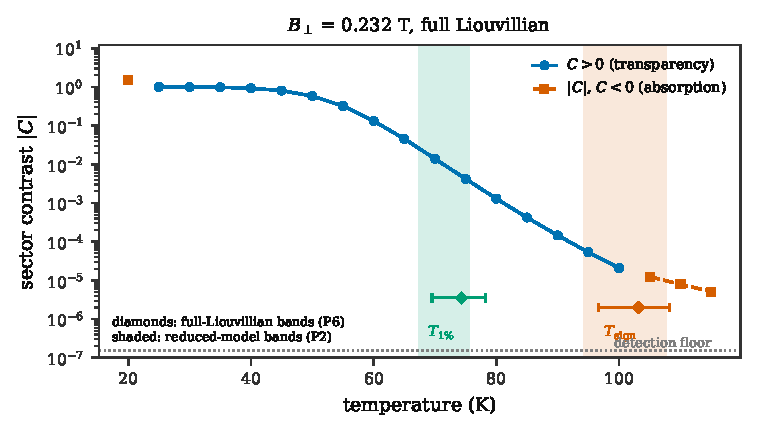
\includegraphics[width=\columnwidth]{fig4_contrast_vs_T.pdf}
\caption{Signed contrast against temperature at
$\Bperp=\SI{0.232}{\tesla}$ from the full Liouvillian; filled circles are
$C>0$, open squares $|C|$ with $C<0$. Shaded bands are the reduced-model 68\%
intervals for $T_{1\%}$ and $T_{\mathrm{sign}}$; diamonds are the
corresponding full-Liouvillian intervals. The dotted line is the contrast
detection floor.}
\label{fig:contrast}
\end{figure}

% ===========================================================================
\section{What an experiment would see}
\label{sec:observables}
% ===========================================================================

Contrast is not an observable. Converting it into one requires a detection
chain, and the conversion must use the same chain at every temperature or the
comparison measures the sample rather than the physics. This is a real
hazard here: the sector cross-section grows as the optical line narrows, so a
fixed sample that is nearly transparent at room temperature
($\mathrm{OD}\approx0.04$) is opaque at \SI{10}{\kelvin}
($\mathrm{OD}\approx16$). We therefore report the optical-depth-matched
sample, $\mathrm{OD}_{\mathrm{sector}}=1$, as the common axis, and record the
required sample length alongside.

We convert to two readouts. Transmission gives
$\Delta T/T=\mathrm{expm1}(\Delta\mathrm{OD})$ with
$\Delta\mathrm{OD}=\mathrm{OD}_{\mathrm{sector}}\,C$. Fluorescence, which for
NV ensembles is often the more practical channel and which has not previously
been evaluated for this system, follows from the change in absorbed power;
in the optically thin limit $\Delta\mathrm{PL}/\mathrm{PL}\to-C$, so a
transparency appears as a fluorescence \emph{dip} of the same fractional size.
Both are propagated to the integration time needed for a signal-to-noise ratio
of five, with shot noise and a relative technical-noise floor of $10^{-6}$.

The outcome, Fig.~\ref{fig:obs}, is that the interesting physics is
observable and the room-temperature limit is not. At \SI{70}{\kelvin} the
transmission signal is $1.4\times10^{-2}$ and needs microseconds. At
\SI{90}{\kelvin} it is $1.5\times10^{-4}$ and needs \SI{10}{\milli\second}. At
\SI{105}{\kelvin}, past the sign reversal, it is $-1.2\times10^{-5}$ and needs
\SI{1.6}{\second}; at \SI{110}{\kelvin}, \SI{5.6}{\second}. The predicted
inversion is thus not a formal remark about a vanishing quantity but a
measurement of a few seconds, with the sign of the fringe as the signature.
Beyond \SI{120}{\kelvin} the technical-noise floor makes the signal
unreachable at any integration time, and at \SI{300}{\kelvin} the residual
contrast of $1.1\times10^{-9}$ is nine orders of magnitude below what the
chain can resolve. Fluorescence tracks transmission up to \SI{105}{\kelvin}
and then falls away first, because a sample thick enough to absorb strongly is
also one whose fluorescence saturates against further changes in absorption.

\begin{figure*}[t]
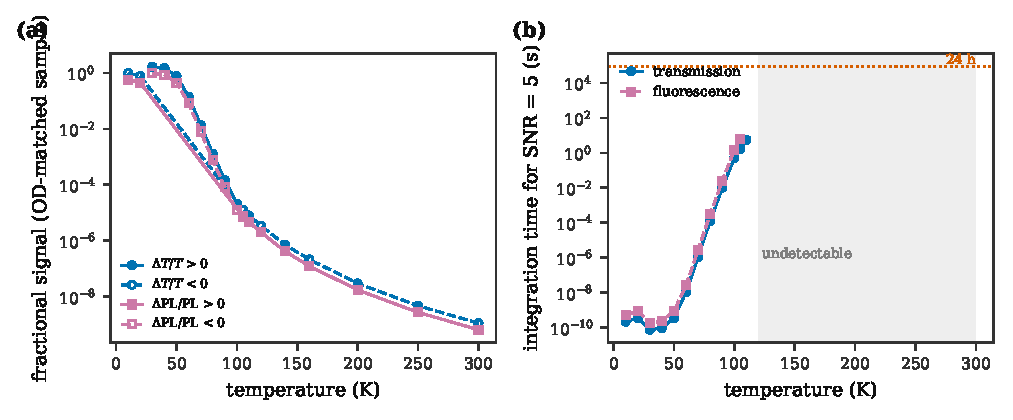
\includegraphics[width=\textwidth]{fig6_observables.pdf}
\caption{(a) Fractional transmission and fluorescence signals against
temperature for the optical-depth-matched sample; filled symbols positive,
open symbols negative. (b) Integration time for SNR${}=5$ in each readout,
with the \SI{24}{\hour} ceiling marked. The sign reversal near
\SI{103}{\kelvin} lies inside the detectable region; the room-temperature
residual does not.}
\label{fig:obs}
\end{figure*}

% ===========================================================================
\section{Model audit}
\label{sec:audit}
% ===========================================================================

\emph{Reduced versus full description.} Much of the literature estimate for
systems of this kind, and our own uncertainty propagation, uses a reduced
kernel in which the excited manifold is handled through a resolvent rather
than by solving the full Liouvillian. Comparing the two on $108$ points of the
$(T,\Bperp)$ plane, they agree to within 10\% at $47$ of them and disagree in
sign at $13$. The disagreements are structured, not random: they concentrate
below \SI{40}{\kelvin}, where the reduced kernel reports transparency
($C\approx+0.99$ at \SI{20}{\kelvin}) while the full Liouvillian reports
control-induced absorption ($C\approx-1.5$), and above \SI{90}{\kelvin}, where
no field gives agreement within 10\%. The reduced kernel is accordingly used
in this work for one purpose only --- the threshold locations of
Sec.~\ref{sec:boundary}, which we verified independently against the full
model --- and every contrast magnitude reported here is from the full
Liouvillian.

\emph{Truncation.} Adding the singlet as a tenth level, or averaging over the
$^{14}$N hyperfine manifold, changes the peak contrast by at most 30\% across
\SI{25}{\kelvin}--\SI{105}{\kelvin} and never changes its sign. Contrast
magnitudes should therefore be read as carrying a structural systematic of
this size; boundary temperatures and the sign reversal are unaffected.

\emph{Classification stability.} At every temperature tested the EIT/ATS
verdict is unchanged under $60$ noise bootstraps at 2\% of the feature depth
and $30$ randomized fit initializations, and under window variations of
$0.5\times$ to $2\times$ in all but one case (\SI{90}{\kelvin}, $3/4$).

\emph{Conventions and provenance.} The sign convention is fixed by
Eq.~\eqref{eq:contrast} and verified directly at the candidate: $C>0$
coincides with $\Afull<\Acut$. Rate conventions follow the $\Gxy/4$ mapping of
Eq.~\eqref{eq:pureloss}. Literature parameters carry recorded sources and
checksums.

\emph{Scope.} The analysis is Markovian, weak-probe, and assumes a unique
steady state. Non-Markovian spectral diffusion enters only through the
effective linewidth prior of Sec.~\ref{sec:boundary}, not as a bath with
memory. Propagation and collective effects are outside the treatment.

% ===========================================================================
\section{Discussion}
% ===========================================================================

The picture that emerges is more constrained than a temperature ceiling. NV
spin-$\Lambda$ EIT occupies a bounded island, and each of its three edges has
a different mechanism: a symmetry obstruction that a transverse field must
lift before there is any channel at all, a control-power crossover into
Autler--Townes splitting at the cold edge, and phonon-driven collapse of the
Raman path at the warm edge. Only the last of these is what the conventional
dephasing argument describes.

This also sharpens what would count as a decisive experiment. A transparency
dip at a single temperature and field establishes little, since a dip is
equally the signature of Autler--Townes splitting; the discriminating
measurements are the quadratic opening with transverse field at the warm end
of the island, the collapse of the contrast with temperature over several
decades, and above all the change of sign near \SI{103}{\kelvin}, which no
Autler--Townes mechanism produces and which we find to be resolvable in
seconds. A measurement that
followed the fringe through zero and out the other side would test the
pathway-interference account directly.

For room temperature the conclusion is negative and, we believe, robust: the
residual contrast is $\sim\!10^{-9}$, nine orders below the detection floor of
a chain that is already optimistic, and it is of the wrong sign in any case.
Reaching a room-temperature solid-state EIT will require a configuration whose
Raman pathway is not damped by an orbital degree of freedom that thermalizes
at these rates --- either a different defect, or NV under conditions that
freeze the orbital dynamics out.

Group-IV centres are the obvious comparison, since their $\Lambda$ channel is
orbital rather than spin and so carries no spin-overlap
obstruction~\cite{B2014A01,L2014A02,I2024S13}; their difficulty is the
opposite one, an orbital ground coherence damped by single-phonon
transitions~\cite{K2015S11}, which strain engineering and larger spin--orbit
splitting are designed to address~\cite{S2018S12,R2021A04}. We treat that
comparison as a design principle rather than a quantitative claim; the
material-independent classification of response orders that would place NV and
group-IV in a common scheme is developed elsewhere.

% ===========================================================================
\section{Conclusion}
% ===========================================================================

We have located the region of the temperature--transverse-field plane in
which the NV$^{-}$ spin-$\Lambda$ channel supports genuine electromagnetically
induced transparency, using the full nine-level Lindblad generator and
classifying by sign, lineshape and an EIT/ATS model comparison together. The
region is a closed island requiring $\Bperp\gtrsim\SI{0.15}{\tesla}$, bounded
below near \SI{22}{\kelvin} and above near \SI{90}{\kelvin}--\SI{95}{\kelvin},
with the contrast falling four and a half orders of magnitude across it. Above
$103\,[97,108]~\si{\kelvin}$ the response inverts to control-induced
absorption, an inversion that a realistic measurement can resolve in seconds
and that constitutes a direct test of the pathway-interference mechanism. At
room temperature the residual response is unobservable by nine orders of
magnitude. We have also delimited the validity of the reduced description
commonly used for such estimates, which reproduces boundary temperatures but
not contrast magnitudes and fails qualitatively outside
\SI{40}{\kelvin}--\SI{90}{\kelvin}.

\begin{acknowledgments}
The author thanks the members of the group for discussions.
\end{acknowledgments}

% Article titles in the reference list.  The revtex4-2 `longbibliography'
% class option is declared but never used by the class, so it cannot switch
% them on; apsrev4-2.bst defaults to title = -1 (disabled).  The working route
% is the @CONTROL entry at the top of references.bib, which BibTeX only reads
% if the entry is cited -- hence the \nocite.  It produces no printed entry.
% The bst consumes the entry without emitting a \bibitem, so natbib would then
% report the key as undefined; predefining its (empty) label silences that
% without typesetting anything, since the key is never \cite'd.
\makeatletter
\expandafter\gdef\csname b@apsrev42Control\endcsname{}
\makeatother
\nocite{apsrev42Control}
\bibliographystyle{apsrev4-2}
\bibliography{references}

\end{document}
